\documentclass{beamer}
%\documentclass[hyperref={pdfpagelabels=false}]{beamer}

\usepackage{graphicx} 
\usepackage[T1]{fontenc}
\usepackage[utf8]{inputenc}
\usepackage[francais]{babel}	

\usetheme{Frankfurt}
\usepackage{lmodern}


\title{Projet: Le Voyageur du Commerce}
\author{Guillaume Aubian}

\date{\today}


\addtobeamertemplate{footline}{\flushright{\insertframenumber/\inserttotalframenumber \hphantom{ba}}}


\begin{document}

%\AtBeginSubsection[]{
 % \begin{frame}<beamer>
    % \frametitle{Outline}
 %    \addtocounter{framenumber}{-1}
 %    \thispagestyle{empty}
  %   \tableofcontents[currentsubsection]
  %\end{frame}
%}

\setbeamertemplate{navigation symbols}{}
\frame{\titlepage}

\section{Le problème}

\begin{frame}{Présentation du problème}
\begin{itemize}
\item Un graphe G ponderé
\item But: Trouver un tour de poids minimal dans G
\item Objectif: minimiser le poids du tour
\end{itemize}
\end{frame}

\begin{frame}{Exemple}
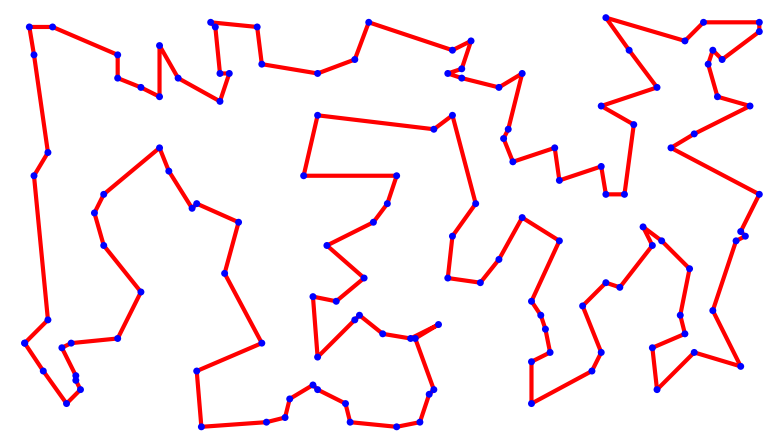
\includegraphics[scale=0.5]{tsp_ex1_2opt.png}
\end{frame}

\section{Le langage}
\begin{frame}{OCaml}
\begin{itemize}
\color{green}
\item Modules
\item Fonctionnel $\rightarrow$ défi!
\color{red}
\item Pas de matrices
\item Difficulté à parser
\end{itemize}
\end{frame}

\begin{frame}{Simplexe}
\begin{itemize}
\item Interêt de la modularité

\item Matrices: obligé de partir de zéro

\item Capable de minimiser/maximiser + inégalités et égalités
\end{itemize}
\end{frame}

\section{Calcul direct du tour}
\begin{frame}{Tour optimal}
\begin{itemize}
\item Module des graphes codé de façon pure

\item Du coup, implémentation de Held-Karp triviale

\item Dynamique avec une table de Hachage
\end{itemize}
\end{frame}

\begin{frame}{Tour approché}
\begin{enumerate}
\item On part d'un tour à un noeud.

\item On le complète à chaque itération

\item Plus possible $\Rightarrow$ fini
\end{enumerate}
Complexité simple/pas de constante absolue $\Rightarrow$ Préféré à l'énoncé
\end{frame}

\section{Utiliser le simplexe pour TSP}
\begin{frame}{Polytope de TSP}
\begin{itemize}
\item On recopie simplement l'énoncé

\item Créer tous les ensembles $\Rightarrow$ Récurrence en $O(2^{n})$

\item Seulement les ensembles ne contenant pas un sommet fixé
\end{itemize}
\end{frame}

\begin{frame}{Coupe Minimale}
On utilise l'algorithme de Stoer-Wagner

\begin{block}{Principe}
$\forall s,t \in V(G),$

$min_{cut}(G) = min (min_{s,t-cut}(G), mincut (G \backslash \{s , t\} \cup \{ merge_{s,t} \}))$

\end{block}

\begin{block}{$min_{s,t-cut}$}
\color{red} Pour G, s et t fixés $\Rightarrow$ flots = lent

\color{green} Pour G, renvoyer s et t $\Rightarrow$ facile 
\end{block}
\end{frame}

\section{Amélioration duale}
\begin{frame}{Dual}
\begin{block}{Problème dual}
\begin{itemize}
\item Trouver une assignation Vrai $\backslash$ Faux (continu) des contraintes

\item $\forall e$, limite sur le nombre de contraintes satisfaites où e apparaît

\item Maximiser la somme pondérée des valeurs associées aux contraintes
\end{itemize}
\end{block}
\end{frame}

\begin{frame}{Idée avec le dual}
\begin{enumerate}
\item On se limite à un sous-ensemble d'arêtes
\item On résout le dual
\item Primal-dual $\Rightarrow$ la solution est optimale?
\item Primal-dual $\Rightarrow$ Quelles contraintes rajouter
\item GoTo 1
\end{enumerate}
\end{frame}

\begin{frame}{Idée avec le dual}
\begin{enumerate}
\item On se limite à un sous-ensemble d'arêtes
\item On résout le dual
\item Primal-dual $\Rightarrow$ la solution est optimale?
\item Primal-dual $\Rightarrow$ Quelles contraintes rajouter
\item GoTo 1
\end{enumerate}

\begin{alertblock}{Malheureusement...}
Pas implémenté
\end{alertblock}
\end{frame}

\section{Questions}
\begin{frame}{PL intégral?}
Non, car:

\begin{itemize}
\item La question suivante n'aurait pas d'interêt
\end{itemize}
\end{frame}

\begin{frame}{PL intégral?}
Non, car:

\begin{itemize}
\item La question suivante n'aurait pas d'interêt
\item Contre-exemple: Graphe complet à 4 noeuds
\end{itemize}
\end{frame}

\begin{frame}{Contre-Exemple}
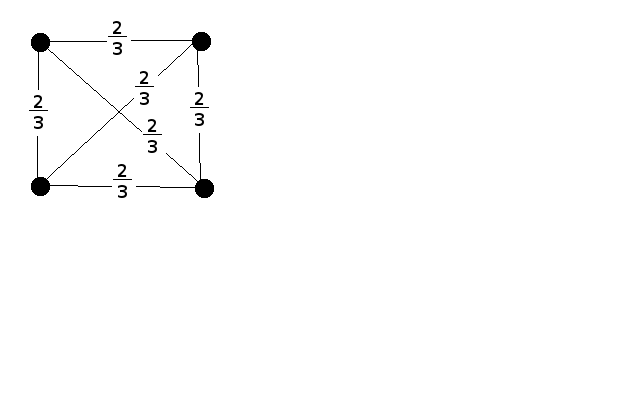
\includegraphics{counter_example.png}
\end{frame}

\begin{frame}{Nouvelles règles?}
\begin{block}{Règle}
$\forall$ cycle propre $C = e_{1} e_{2} ... e_{c}$

$\sum_{i=1}^{c}x_{e_{i}} = c-1$
\end{block}

Beaucoup de cycles $\Rightarrow$ se restreindre aux cycles élémentaires?

\end{frame}

\begin{frame}{Conclusion}
\begin{itemize}
\item Sujet intéressant
\item Déçu de ne pas avoir fini
\item Nouvelles règles?
\item Meilleures performances avec points intérieurs?
\end{itemize}
\end{frame}
\end{document}

